\subsection{Side muon range detector}
Two Side-MRD modules for tracking secondary particles from neutrino interactions will be installed in 2018. 
Each Side-MRD module is composed of 11  steel plates and 10 layers of total 80 scintillator slabs installed  in 13~mm gaps between the 30~mm thick plates. Each steel plate size is  $30\times1610\times1800$ mm$^{3}$. Total module size  is  $2236\times1630\times975$ mm$^{3}$ as shown in Fig. \ref{fig:side_mrd} (left), weight is $\sim$8.5 ton. 

Scintillator bars were manufactured by Uniplast company in Vladimir, Russia. Polystyrene based scintillators were extruded with thickness of 7~mm, then cut to the size of $7\times200\times1800$ mm$^{3}$. Dopant composition is  1.5\% PTP and 0.01\% POPOP.
Scintillator surface was etched by a chemical agent to form a white diffuse layer with excellent reflective performance. 
Ideal contact between the scintillator and the reflector raises the light yield up to 50\% comparing to an uncovered scintillator. 
Sine like groove was milled along the scintillator to provide uniform light collection over the whole scintillator surface. 
WLS Y11 Kuraray fiber of 1 ~mm diameter is glued with an optical cement EJ-500 in the S-shape groove  as shown in Fig. \ref{fig:side_mrd}(right). Bending radius is fixed to  30~mm that was specified to be safe for Kuraray S-type fibers.
Both ends of the fiber are glued into optical connectors %(Fig. \ref{fig:side_mrd_optical_con})
which mounted within a scintillator body and provide an interface to SiPMs, Hamamatsu  MPPC S13081-050CS(X1). 

%The plastic molded connectors provide an interface to SiPMs, Hamamatsu  MPPC S13081-050CS(X1) used for the WAGASCI detector. 
%Optical coupler of this type (so-called Baby-mind type of optical connector) consists of two parts (see Fig. \ref{fig:side_mrd_optical_con}):  an container for the MPPC  and  a ferrule with the fiber.  The ferrule  is glued in the scitillator, and its end with glued in WLS fiber was polished. 
%Both parts of the optical coupler are latched by a snap-like mechanism: a locking groove inside the container and matching ring protuberance on the ferrule.
%To ensure the optical contact a foam spring made of sponge rubber presses the MPPC to the fiber end (Fig. \ref{fig:side_mrd_optical_scheme}). 

\begin{figure}[tbhp]
  \begin{center}
   \begin{subfigure}{0.48\textwidth}
     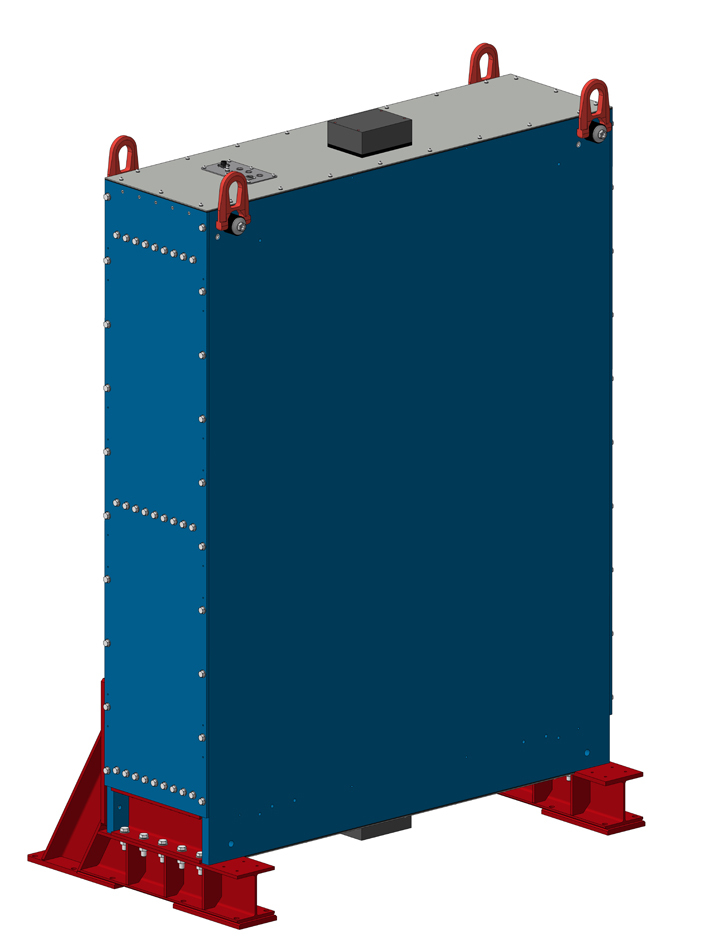
\includegraphics[width=\linewidth]{fig/SMRD_Module.pdf}
    \end{subfigure}
  \begin{subfigure}{0.48\textwidth}
      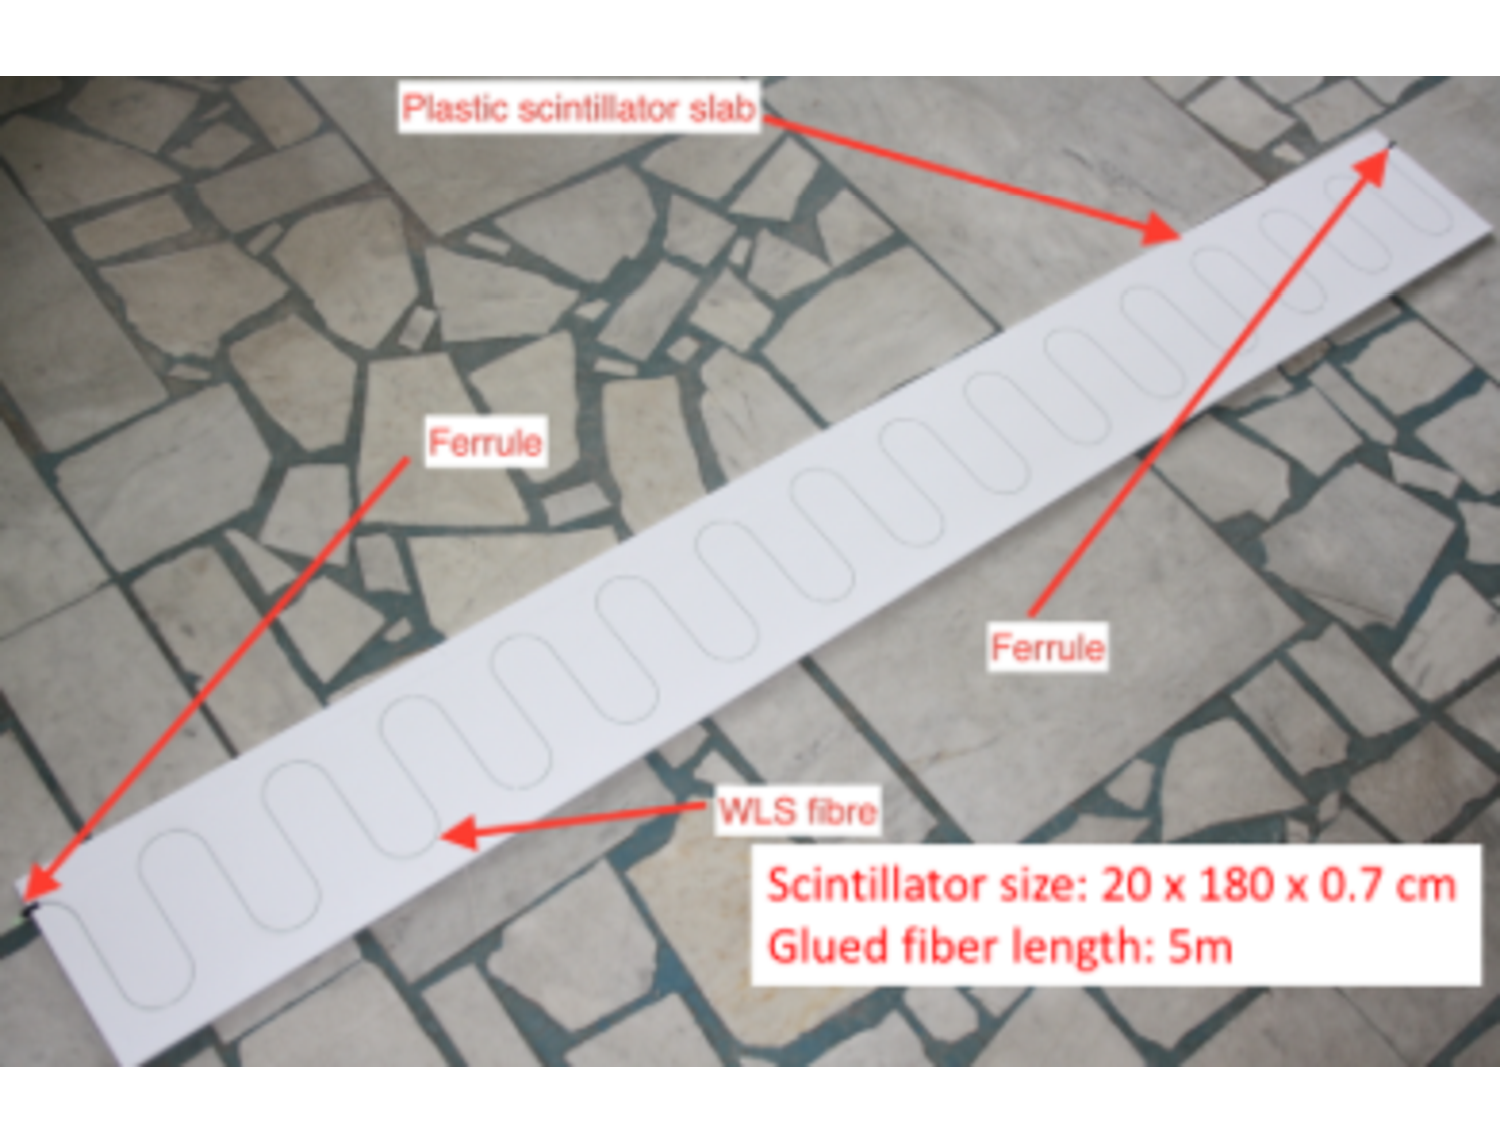
\includegraphics[width=\linewidth]{fig/side_mrd_scintillator.pdf}
    \end{subfigure}    
    \end{center}
  \caption{Left :Side-MRD module. Right: Scintillator bar of the Side-MRD modules.}
\label{fig:side_mrd}
\end{figure}


%\begin{figure}[tbh]
%\begin{center}
%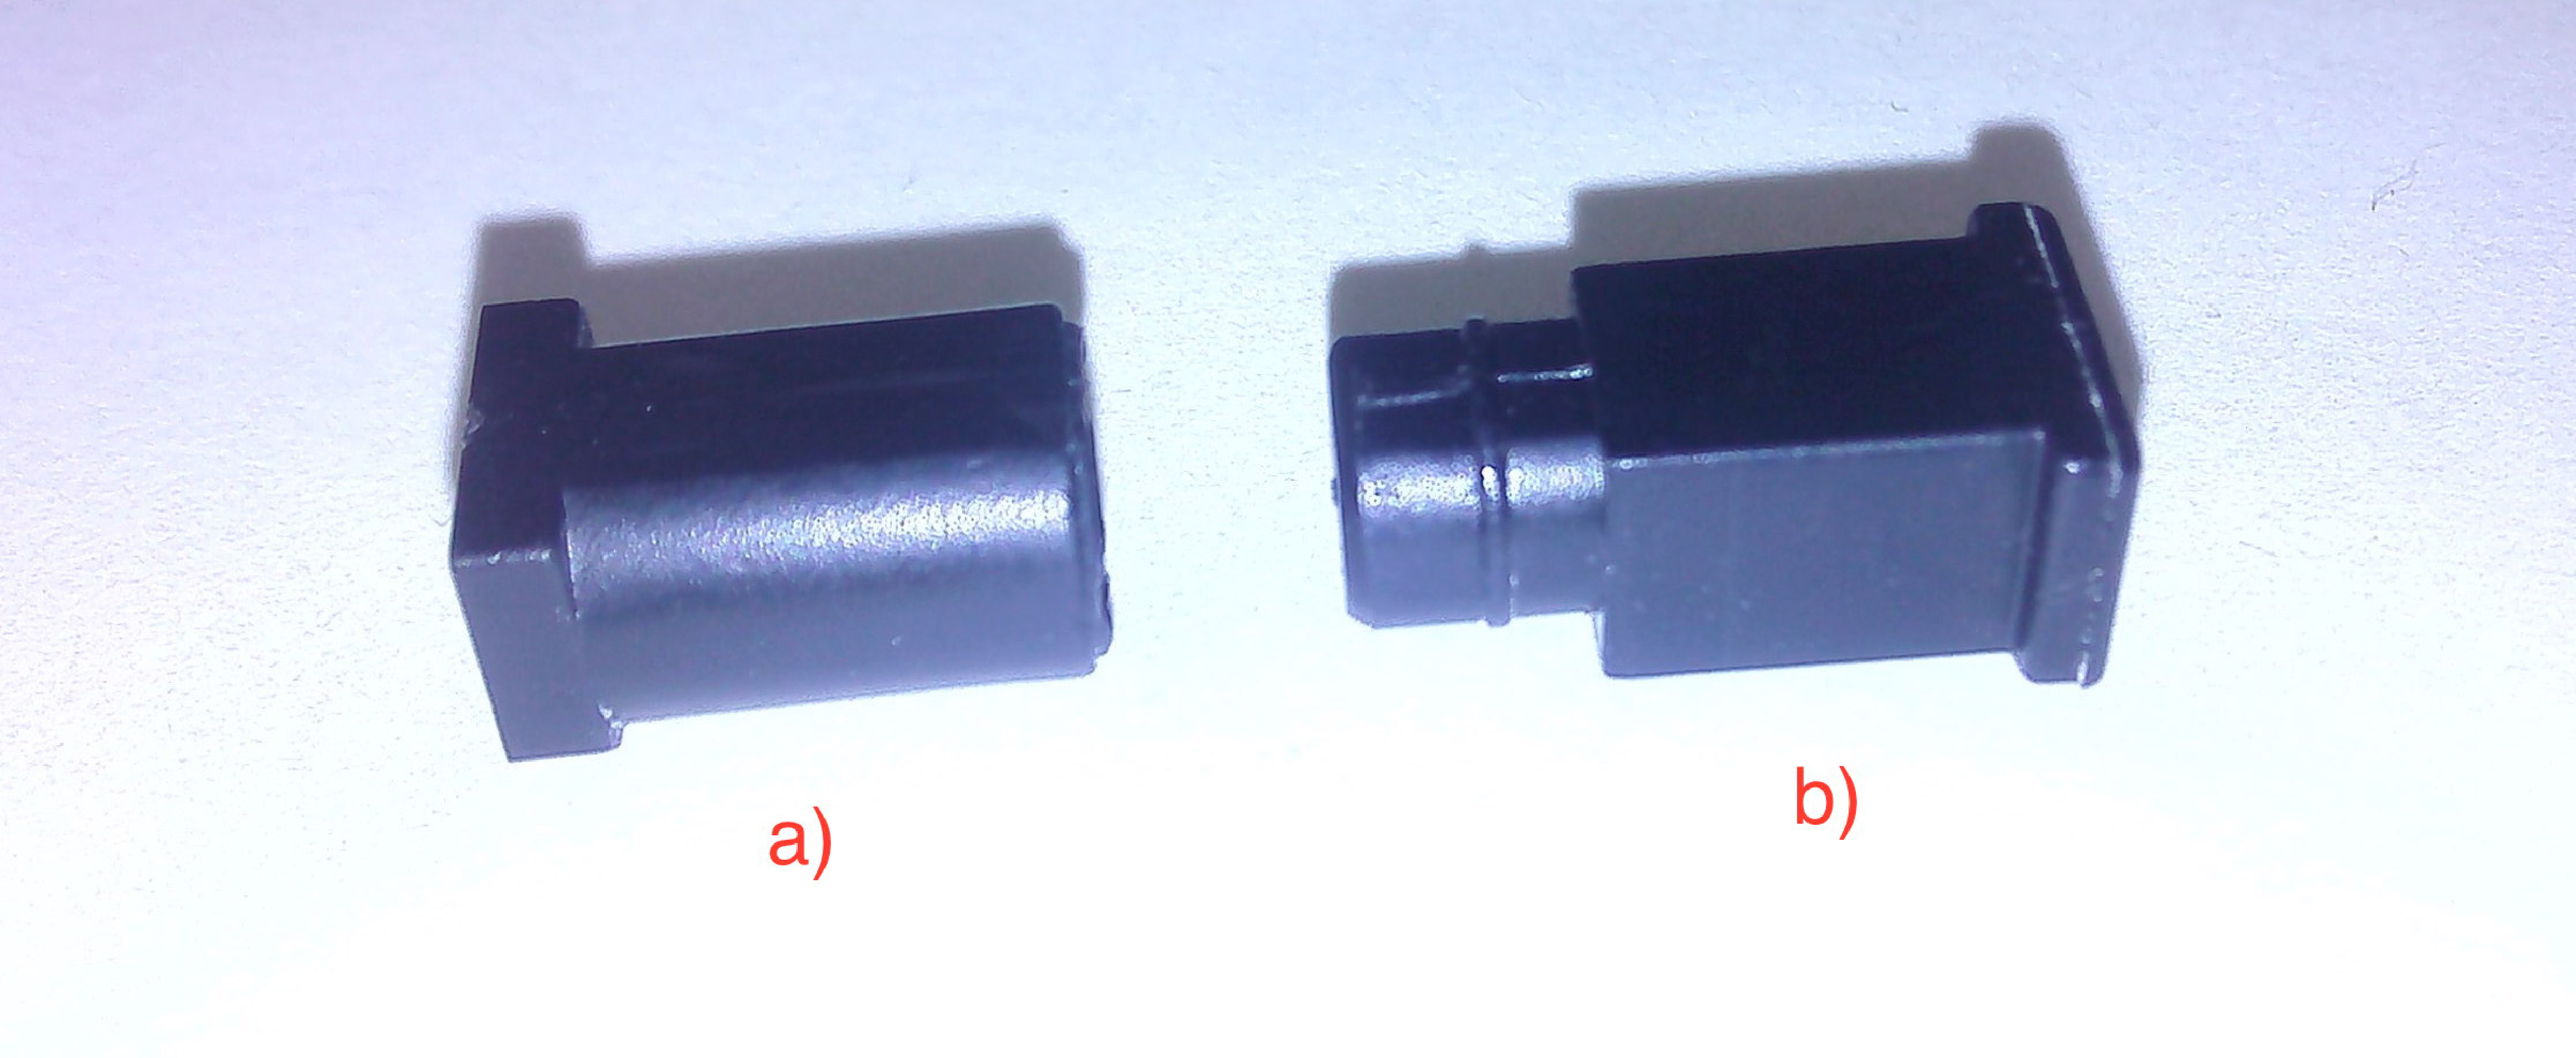
\includegraphics[width=0.8\linewidth]{fig/side_mrd_optical_con.pdf}
%\end{center}
%\caption{
%Optical connector for the Side-MRD scintillator. a) MPPC cover. b) Ferrule.
%}
%\label{fig:side_mrd_optical_con}
%\end{figure}

%\begin{figure}[tbh]
%\begin{center}
%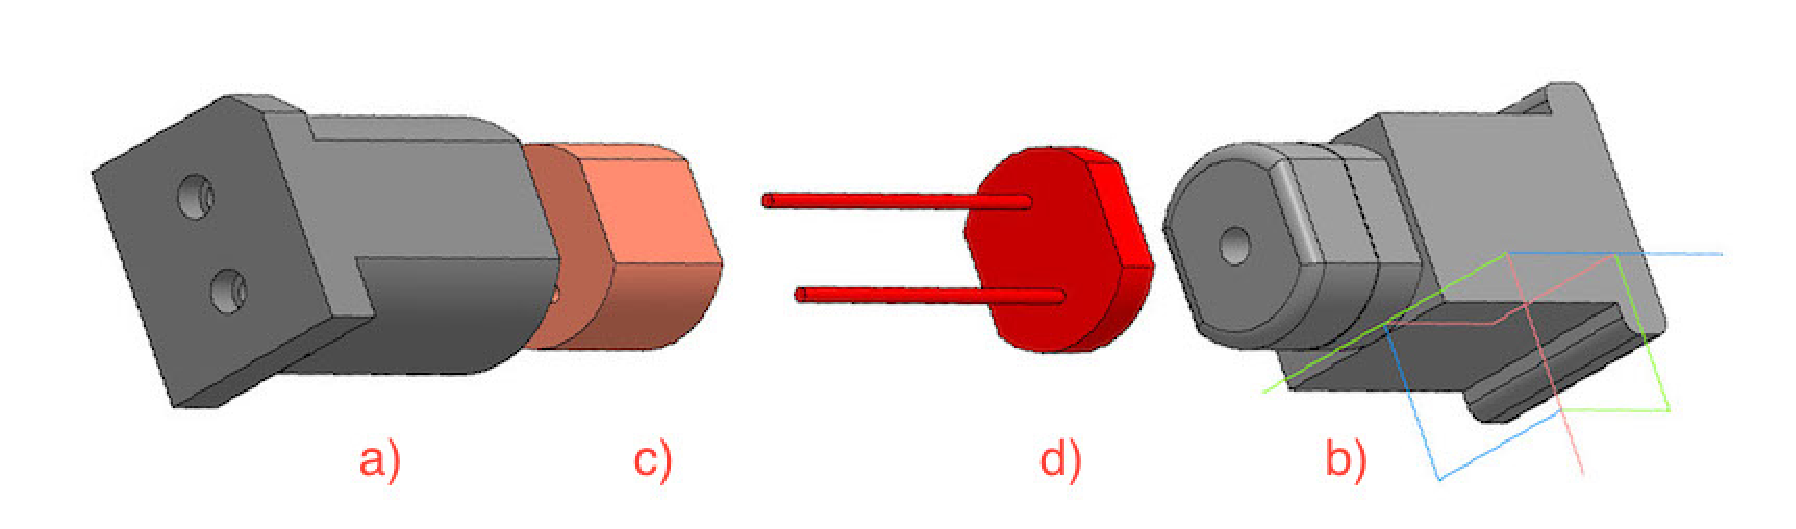
\includegraphics[width=0.8\linewidth]{fig/side_mrd_optical_scheme.pdf}
%\end{center}
%\caption{
%Scheme of the MPPC placement in optical connector.  a) MPPC cover. b) Ferrule. c) Spring (sponge rubber). d) MPPC.
%}
%\label{fig:side_mrd_optical_scheme}
%\end{figure}

Scintillators for the Side-MRD modules had been assembled at INR in Russia, and shipped to Japan in July 2017. The light yield for each scintillator was measured with cosmic rays at INR and at YNU in Japan after delivery.  Parameters measured at the center of the counter were : the light yields  $LY_{1}$ and $LY_{2}$ at both ends, the light yield asymmetry between the ends calculated as $100\% \times \frac{LY_{1}-LY_{2}}{LY_{1}+LY_{2}}$.
After tests at INR we selected 324 counters from measured 332 ones with the mean light yield of 45 p.e./MIP ( $LY_{1}$+ $LY_{2}$ ) and the asymmetry value less than 10 \% . 
The measuremens at YNU yielded the average total light yield of about 40 p.e./MIP which varies in range  from 32 to 50 p.e/MIP  (Fig. \ref{fig:side_mrd_ly} (left)). Only two counters  showed relatively high asymmetry close to 25 \% as shown in Fig. \ref{fig:side_mrd_ly} (right). 
Using the results of the quality assurance test  we selected 320 scintillator counters for the Side-MRD modules. 

We also measured the time resolution for a combination of four  counters piled each on another one.
%Time resolution for a single counter is determined as rms of $(T_{left}-T{right})/2$ distribution. The difference of times was chosen to remove the correlated time fluctuation caused by a start trigger signal.
The average result for four counters is  $\sigma_T$ = 1.04~ns. %(Upper left plot in Fig. \ref{fig:side_mrd_combi_time}). 
%For a set of $n$ counters the time resolution is calculated as $\frac{(T_{L}-T_{R})_{1}+(T_{L}-T_{R})_{2}+...+(T_{L}-T_{R})_{n}}{2 \times n}$. The result of combination of 2, 3, 4 counters is 0.79~ns, 0.66~ns and 0.58~ns, correspondently (Fig. \ref{fig:side_mrd_combi_time}).
The resolution of combination of 2, 3, 4 counters is measured to be 0.79~ns, 0.66~ns and 0.58~ns, correspondently.
\begin{figure}[tbh]
\begin{center}
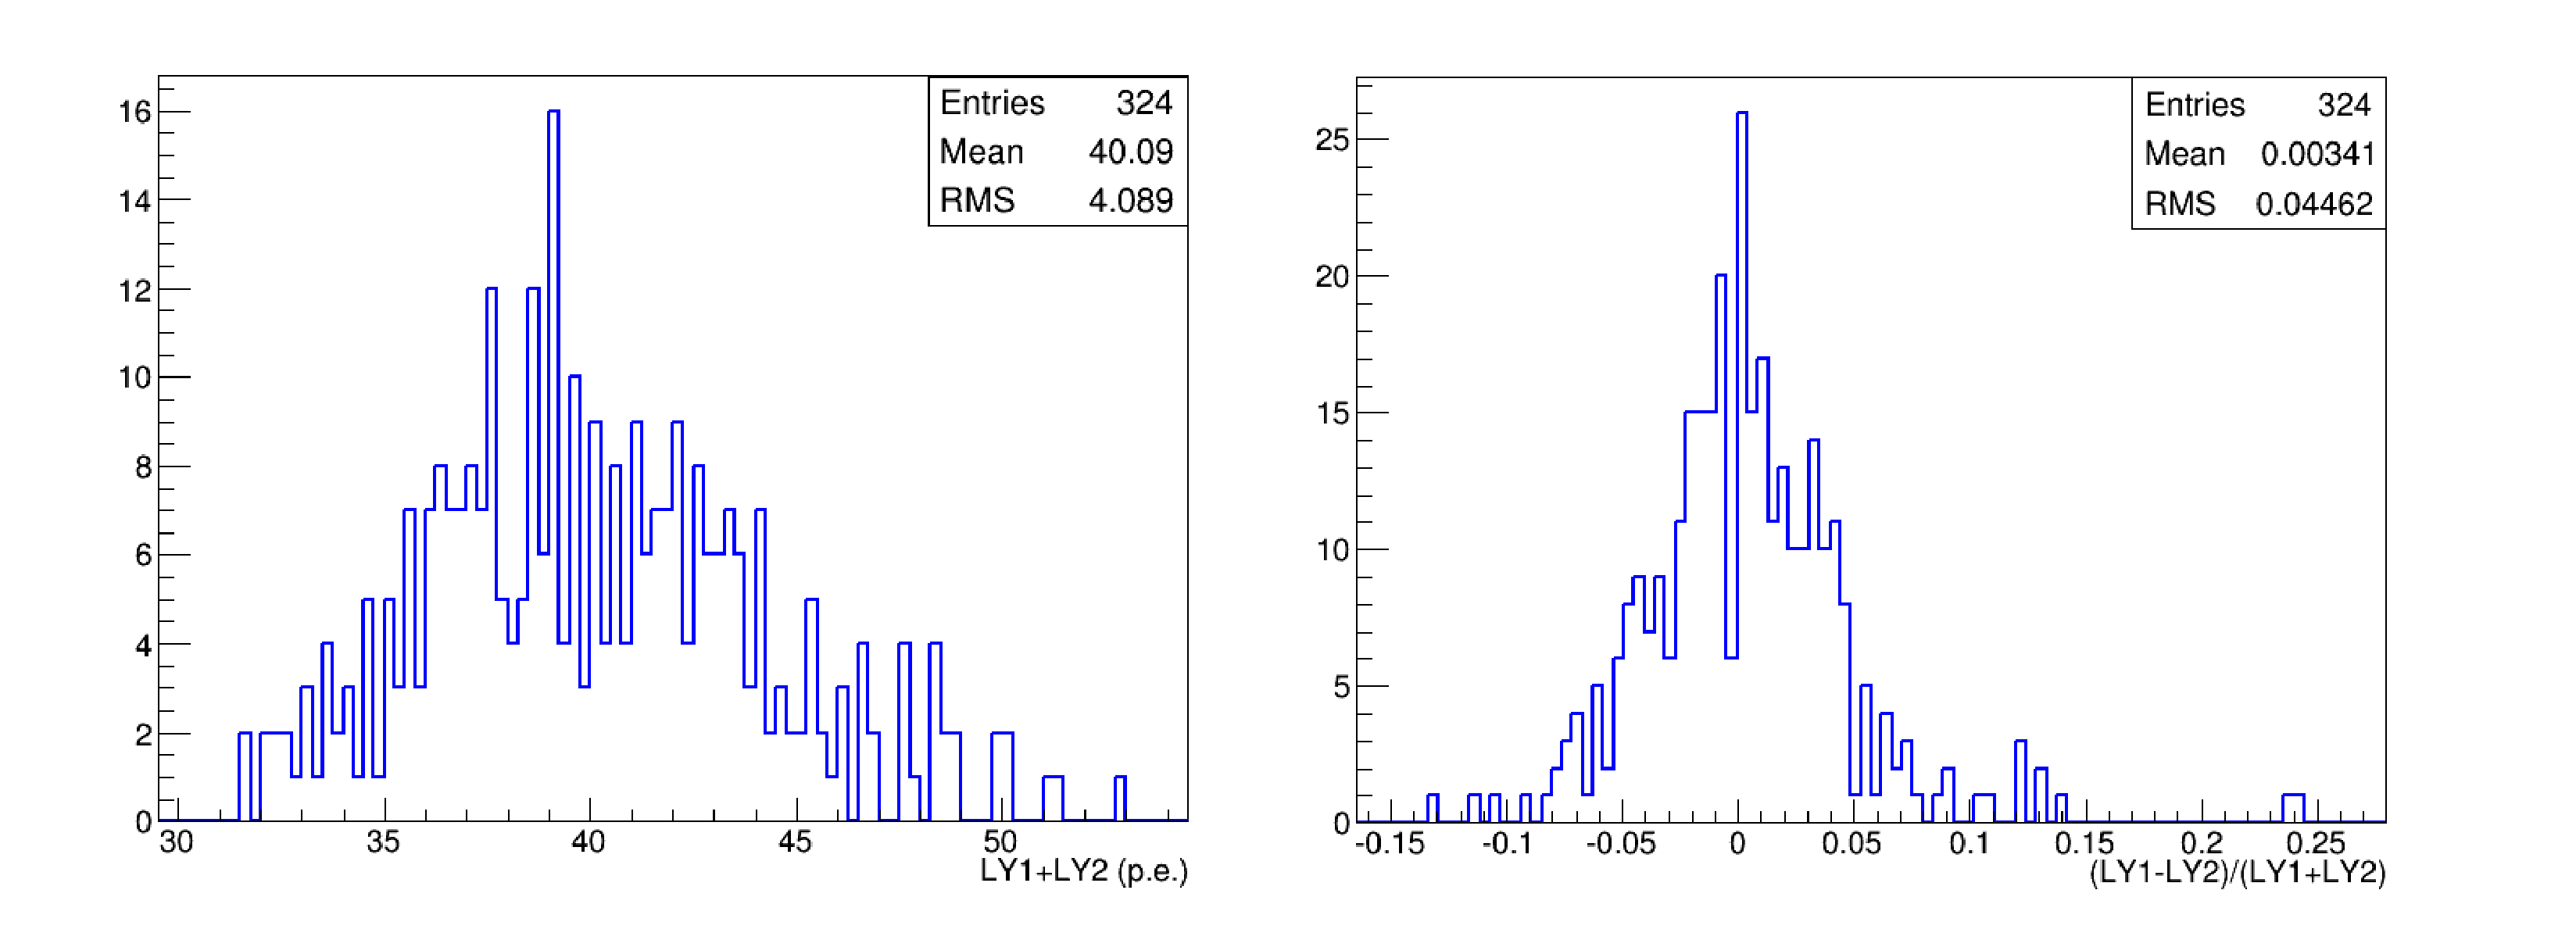
\includegraphics[width=0.8\linewidth]{fig/side_mrd_ly.pdf}
\end{center}
\caption{
Total light yield distribution (left) and light yield assymetry (right) measured at YNU.
}
\label{fig:side_mrd_ly}
\end{figure}

%\begin{figure}[tbh]
%\begin{center}
%\includegraphics[width=0.8\linewidth]{fig/side_mrd_combi_time.pdf}
%\end{center}
%\caption{
%Time resolution for one (upper left) and a set of 2,3,4 Side-MRD counters.
%}
%\label{fig:side_mrd_combi_time}
%\end{figure}
Construction of Side-MRD modules will be done from November 2017 at Yokohama National University, then they will be transported to J-PARC and will be installed at  B2 floor of the T2K near detector hall.% before  T2K beam in March 2018.
